Writing an in-tree LLVM IR regression test is pretty easy: all you need to do is annotate the IR file with testing directives. Look at the following script, for example:

\begin{tcolorbox}[colback=white,colframe=black]
\tt
\zihao{-5}
; RUN: opt < \%s -instcombine -S -o - | FileCheck \%s \\
target triple = "x86\_64-unknown-linux" \\
define i32 @foo(i32 \%c) \{ \\
\hspace*{0.3cm}entry: \\
\hspace*{0.3cm}; CHECK: [[RET:\%.+]] = add nsw i32 \%c, 3 \\
\hspace*{0.3cm}; CHECK: ret i32 [[RET]] \\
\hspace*{0.3cm}\%add1 = add nsw i32 \%c, 1 \\
\hspace*{0.3cm}\%add2 = add nsw i32 \%add1, 2 \\
\hspace*{0.3cm}ret i32 \%add2 \\
\}
\end{tcolorbox}

This script checks if InstCombine (triggered by the -instcombine command-line option shown in the preceding snippet) simplifies two succeeding arithmetic adds into one. After putting this file into an arbitrary folder under llvm/test, the script will automatically be picked and run as part of the regression test when you're executing the llvm-lit command-line tool.

Despite its convenience, this barely helps you use LIT in out-of-tree projects. Using LIT out-of-tree is especially useful when your project needs some end-to-end testing facilities, such as a format converter, a text processor, a linter, and, of course, a compiler. This section will show you how to bring LIT to your out-of-tree projects, and then provide you with a complete picture of the running flow of LIT.

\subsubsubsection{3.2.1\hspace{0.2cm}Preparing for our example project}

In this section, we will use an out-of-tree CMake project. This example project builds a command-line tool, js-minifier, that minifies arbitrary JavaScript code. We will transform the following JavaScript code:

\begin{lstlisting}[style=styleJavaScript]
const foo = (a, b) => {
	let c = a + b;
	console.log(`This is ${c}`);
}
\end{lstlisting}

This will be transformed into some other semantic-equivalent code that is as short as possible:

\begin{lstlisting}[style=styleJavaScript]
const foo = (a,b) => {let c = a + b; console.log(`This is ${c}`);}
\end{lstlisting}

Instead of teaching you how to write this js-minifier, the goal of this section is to
show you how to create a LIT testing environment to test this tool.

The example project has the following folder structure:

\begin{tcolorbox}[colback=white,colframe=black]
\tt
\zihao{-5}
/JSMinifier \\
\hspace*{0.3cm}|\_\_\_ CMakeLists.txt \\
\hspace*{0.3cm}|\_\_\_ /src \\
\hspace*{0.3cm}|\hspace{1cm}|\_\_\_ js-minifier.cpp \\
\hspace*{0.3cm}|\hspace{1cm}|\_\_\_ /test \\
\hspace*{0.3cm}|\hspace{2.3cm}|\_\_\_ test.js \\
\hspace*{0.3cm}|\hspace{2.3cm}|\_\_\_ CMakeLists.txt \\
\hspace*{0.3cm}|\_\_\_ /build
\end{tcolorbox}

The files under the /src folder contain the source code for js-minifier (which we are not going to cover here). What we will focus on here are the files that will be used for testing js-minifier, which sit under the /test folder (for now, there is only one file, test.js).

In this section, we are going to set up a testing environment so that when we run llvmlit – the testing driver and main character of this section – under the CMake /build folder, it will print testing results, like this:

\begin{tcblisting}{commandshell={}}
$ cd build
$ llvm-lit -sv .
-- Testing: 1 tests, 1 workers –
PASS: JSMinifier Test :: test.js (1 of 1)
Testing Time: 0.03s
  Expected Passes : 1
\end{tcblisting}

This shows how many and what test cases have passed.

Here is the testing script, test.js:

\begin{lstlisting}[style=styleJavaScript]
// RUN: %jsm %s -o - | FileCheck

// CHECK: const foo = (a,b) =>
// CHECK-SAME: {let c = a + b; console.log(`This is ${c}`);}
const foo = (a, b) => {
	let c = a + b;
	console.log(`This is ${c}`);
}
\end{lstlisting}

As you can see, it is a simple testing process that runs the js-minifier tool – represented by the \texttt{\%jsm} directive, which will be replaced by the real path to js-minifier executable, as explained later – and checks the running result with FileCheck by using its CHECK and CHECK-SAME directives.

With that, we've set up our example project. Before we wrap up the preparation, there is one final tool we need to create.

Since we're trying to cut down on our reliance on the LLVM source tree, recreate the llvm-lit command-line tool using the LIT package available in the PyPi repository (that is, the pip command-line tool). All you need to do is install that package:

\begin{tcblisting}{commandshell={}}
$ pip install --user lit
\end{tcblisting}

Finally, wrap the package with the following script:

\begin{lstlisting}[style=stylePython]
#!/usr/bin/env python
from lit.main import main
if __name__ == '__main__':
	main()
\end{lstlisting}

Now, we can use LIT without building an LLVM tree! Next, we will create some LIT configuration scripts that will drive the whole testing flow.

\subsubsubsection{3.2.2\hspace{0.2cm}Writing LIT configurations}

In this subsection, we'll show you how to write LIT configuration scripts. These scripts describe the testing process – where the files will be tested, the testing environment (if we need to import any tool, for example), the policy when there is a failure, and so on. Learning these skills can greatly improve how you use LIT in places outside the LLVM tree. Let's get started:

\begin{enumerate}
\item Inside the /JSMinifier/test folder, create a file called lit.cfg.py that contains the following content:

\begin{lstlisting}[style=stylePython]
import lit.formats

config.name = 'JSMinifier Test'
config.test_format = lit.formats.ShTest(True)
config.suffixes = ['.js']
\end{lstlisting}

Here, the snippet is providing LIT with some information. The config variable here is a Python object that will be populated later when this script is loaded into LIT's runtime. It's basically a registry with predefined fields that carry configuration values, along with custom fields that can be added by lit.*.py scripts at any time.

The config.test\_format field suggests that LIT will run every test inside a shell environment (in the ShTest format), while the config.suffixes field suggests that only files with .js in their filename suffix will be treated as test cases (that is, all the JavaScript files).

\item Following on from the code snippet in the previous step, LIT now needs two other pieces of information: the root path to the test files and the working directory:

\begin{lstlisting}[style=stylePython]
…
config.suffixes = ['.js']
config.test_source_root = os.path.dirname(__file__)
config.test_exec_root = os.path.join(config.my_obj_root,
'test')
\end{lstlisting}

For config.test\_source\_root, it's simply pointing to /JSMinifier/test. On the other hand, config.test\_exec\_root, which is the working directory, is pointing to a place whose parent folder is the value of a custom configuration field, my\_obj\_root. While it will be introduced later, simply put, it points to the build folder path. In other words, config.test\_exec\_root will eventually have a value of /JSMinifier/build/test.

\item The \%jsm directive we saw earlier in test.js is used as a placeholder that will eventually be replaced with the real/absolute path of the js-minifier executable. The following lines will set up the replacements:

\begin{lstlisting}[style=stylePython]
…
config.test_exec_root = os.path.join(config.my_obj_root, 'test')

config.substitutions.append(('%jsm',
os.path.join(config.my_obj_root, 'js-minifier')))
\end{lstlisting}

This code adds a new entry to the config.substitutions field, which makes LIT replace every \%jsm occurrence in the test files with the /JSMinifier/ build/js-minifier value. This wraps up all the content in lit.cfg.py.

\item Now, create a new file called lit.site.cfg.py.in and put it under the /JSMinifier/test folder. The first part of this file looks like this:

\begin{lstlisting}[style=stylePython]
import os
config.my_src_root = r'@CMAKE_SOURCE_DIR@'
config.my_obj_root = r'@CMAKE_BINARY_DIR@'
\end{lstlisting}

The mystery config.my\_obj\_root field is finally resolved here, but instead of pointing to a normal string, it is assigned to a weird value called @CMAKE\_BINARY\_DIR@. Again, this will be replaced by CMake with the real path later. The same goes for the config.my\_src\_root field.

\item Finally, lit.site.cfg.py.in is wrapped up by these lines:

\begin{lstlisting}[style=stylePython]
…
lit_config.load_configure(
	config, os.path.join(config.my_src_root, 'test/
		lit.cfg.py'))
\end{lstlisting}

Even though this snippet is pretty simple, it's a little hard to understand. Simply put, this file will eventually be materialized into another file, with all the variables clamped by @ being resolved and copied into the build folder. From there, it will call back the lit.cfg.py script we saw in the earlier steps. This will be explained later in this section.

\item Finally, it's time to replace those weird @-clamped strings with real values using CMake's configure\_file function. In /JSMinifier/test/CMakeLists.txt, add the following line somewhere inside the file:

\begin{lstlisting}[style=styleCMake]
configure_file(lit.site.cfg.py.in
lit.site.cfg.py @ONLY)
\end{lstlisting}

The configure\_file function will replace all the @-clamped string occurrences in the input file (lit.site.cfg.py.in, in this case) with their CMake variable counterparts in the current CMake context.

For example, let's say there is a file called demo.txt.in that contains the following content:

\begin{lstlisting}[style=styleCMake]
name = "@FOO@"
age = @AGE@
\end{lstlisting}

Now, let's use configure\_file in CMakeLists.txt:

\begin{lstlisting}[style=styleCMake]
set(FOO "John Smith")
set(AGE 87)
configure_file(demo.txt.in
			   demo.txt @ONLY)
\end{lstlisting}

Here, the aforementioned replacement will kick in and generate an output file, demo.txt, that contains the following content:

\begin{lstlisting}[style=styleCMake]
name = "John Smith"
age = 87
\end{lstlisting}

\item Back to the lit.site.cfg.py.in snippets, since CMAKE\_SOURCE\_DIR and CMAKE\_BINARY\_DIR are always available, they point to the root source folder and the build folder, respectively. The resulting /JSMinifier/build/test/lit. site.cfg.py will contain the following content:

\begin{lstlisting}[style=stylePython]
import os
config.my_src_root = r'/absolute/path/to/JSMinifier'
config.my_obj_root = r'/absolute/path/to/JSMinifier/build'

lit_config.load_config(
	config, os.path.join(config.my_src_root, 'test/
		lit.cfg.py'))
\end{lstlisting}

\end{enumerate}

With that, we have learned how to write LIT configuration scripts for our example project. Now, it is time to explain some details of how LIT works internally, and why we need so many files (lit.cfg.py, lit.site.cfg.py.in, and lit.site.cfg.py).

\subsubsubsection{3.2.3\hspace{0.2cm}LIT internals}

Let's look at the following diagram, which illustrates the workflow of running LIT tests in the demo project we just created:

\hspace*{\fill} \\ %插入空行
\begin{center}
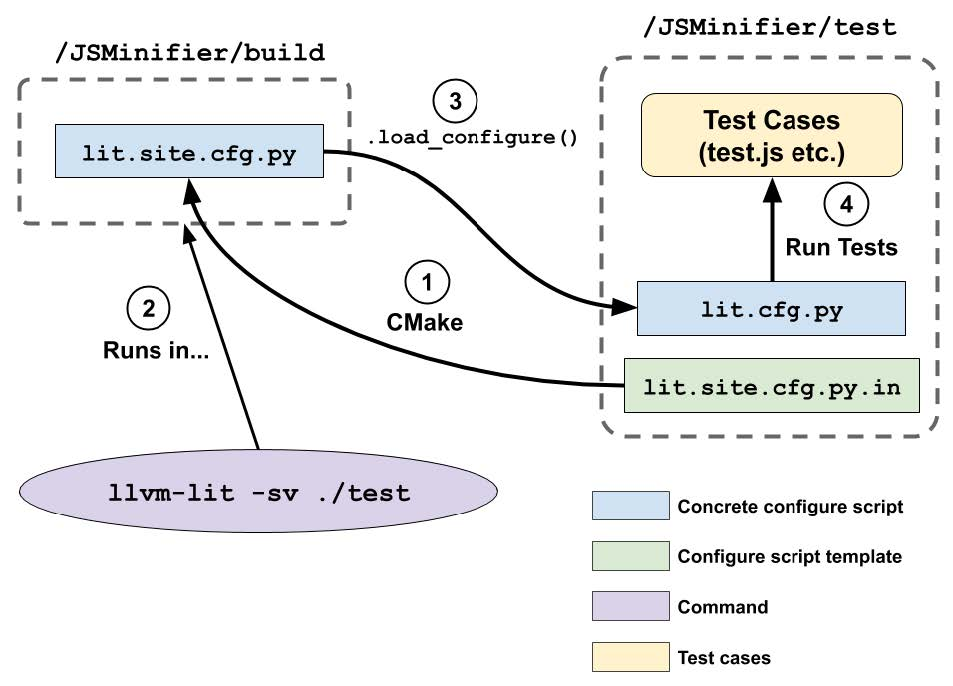
\includegraphics[width=0.8\textwidth]{content/1/chapter3/images/1.jpg}\\
Figure 3.1 – The forking flow of LIT in our example project
\end{center}

Let's take a look at this diagram in more detail:

\begin{enumerate}
\item lit.site.cfg.py.in is copied to /JSMinifier/build/lit.site.cfg.py, which carries some CMake variable values.
\item The llvm-lit command is launched inside /JSMinifier/build. It will execute lit.site.cfg.py first.
\item lit.site.cfg.py then uses the load\_configure Python function to load the main LIT configurations (lit.cfg.py) and run all the test cases.
\end{enumerate}

The most crucial part of this diagram is explaining the roles of lit.site.cfg.py and lit.site.cfg.py.in: many parameters, such as the absolute path to the build folder, will remain unknown until the CMake configuration process is complete. So, a trampoline script – that is, lit.site.cfg.py – is placed inside the build folder to relay that information to the real test runner.

In this section, we learned how to write LIT configuration scripts for our out-of-tree example project. We also learned how LIT works under the hood. Knowing this can help you use LIT in a wide variety of projects, in addition to LLVM. In the next section, we will focus on FileCheck, a crucial and commonly used LIT utility that performs advanced pattern checking.





